\chapter{Additional plots for all simulations}

\label{A:allres}
This Appendix contains additional plots showing combined results of Simulation Study 1 described in Chapter \ref{C:chap_sim2} and Simulation Study 2 described in Chapter \ref{C:chap_sim3}. Based on Section \ref{S:chap_intro:correlation} and \cite{Ciani2014} only results for a realistic range for the correlation between time to progression and overall survival are presented in this Appendix. That is only the correlations of 0.4, 0.6 and 0.8 are presented here. Care should be taken when examining these plots as the y axis are not constant. Table \ref{T:chap_con:scenarios} shows the description for each of the 21 basis scenarios.

\clearpage

\begin{sidewaysfigure}
    \centering
    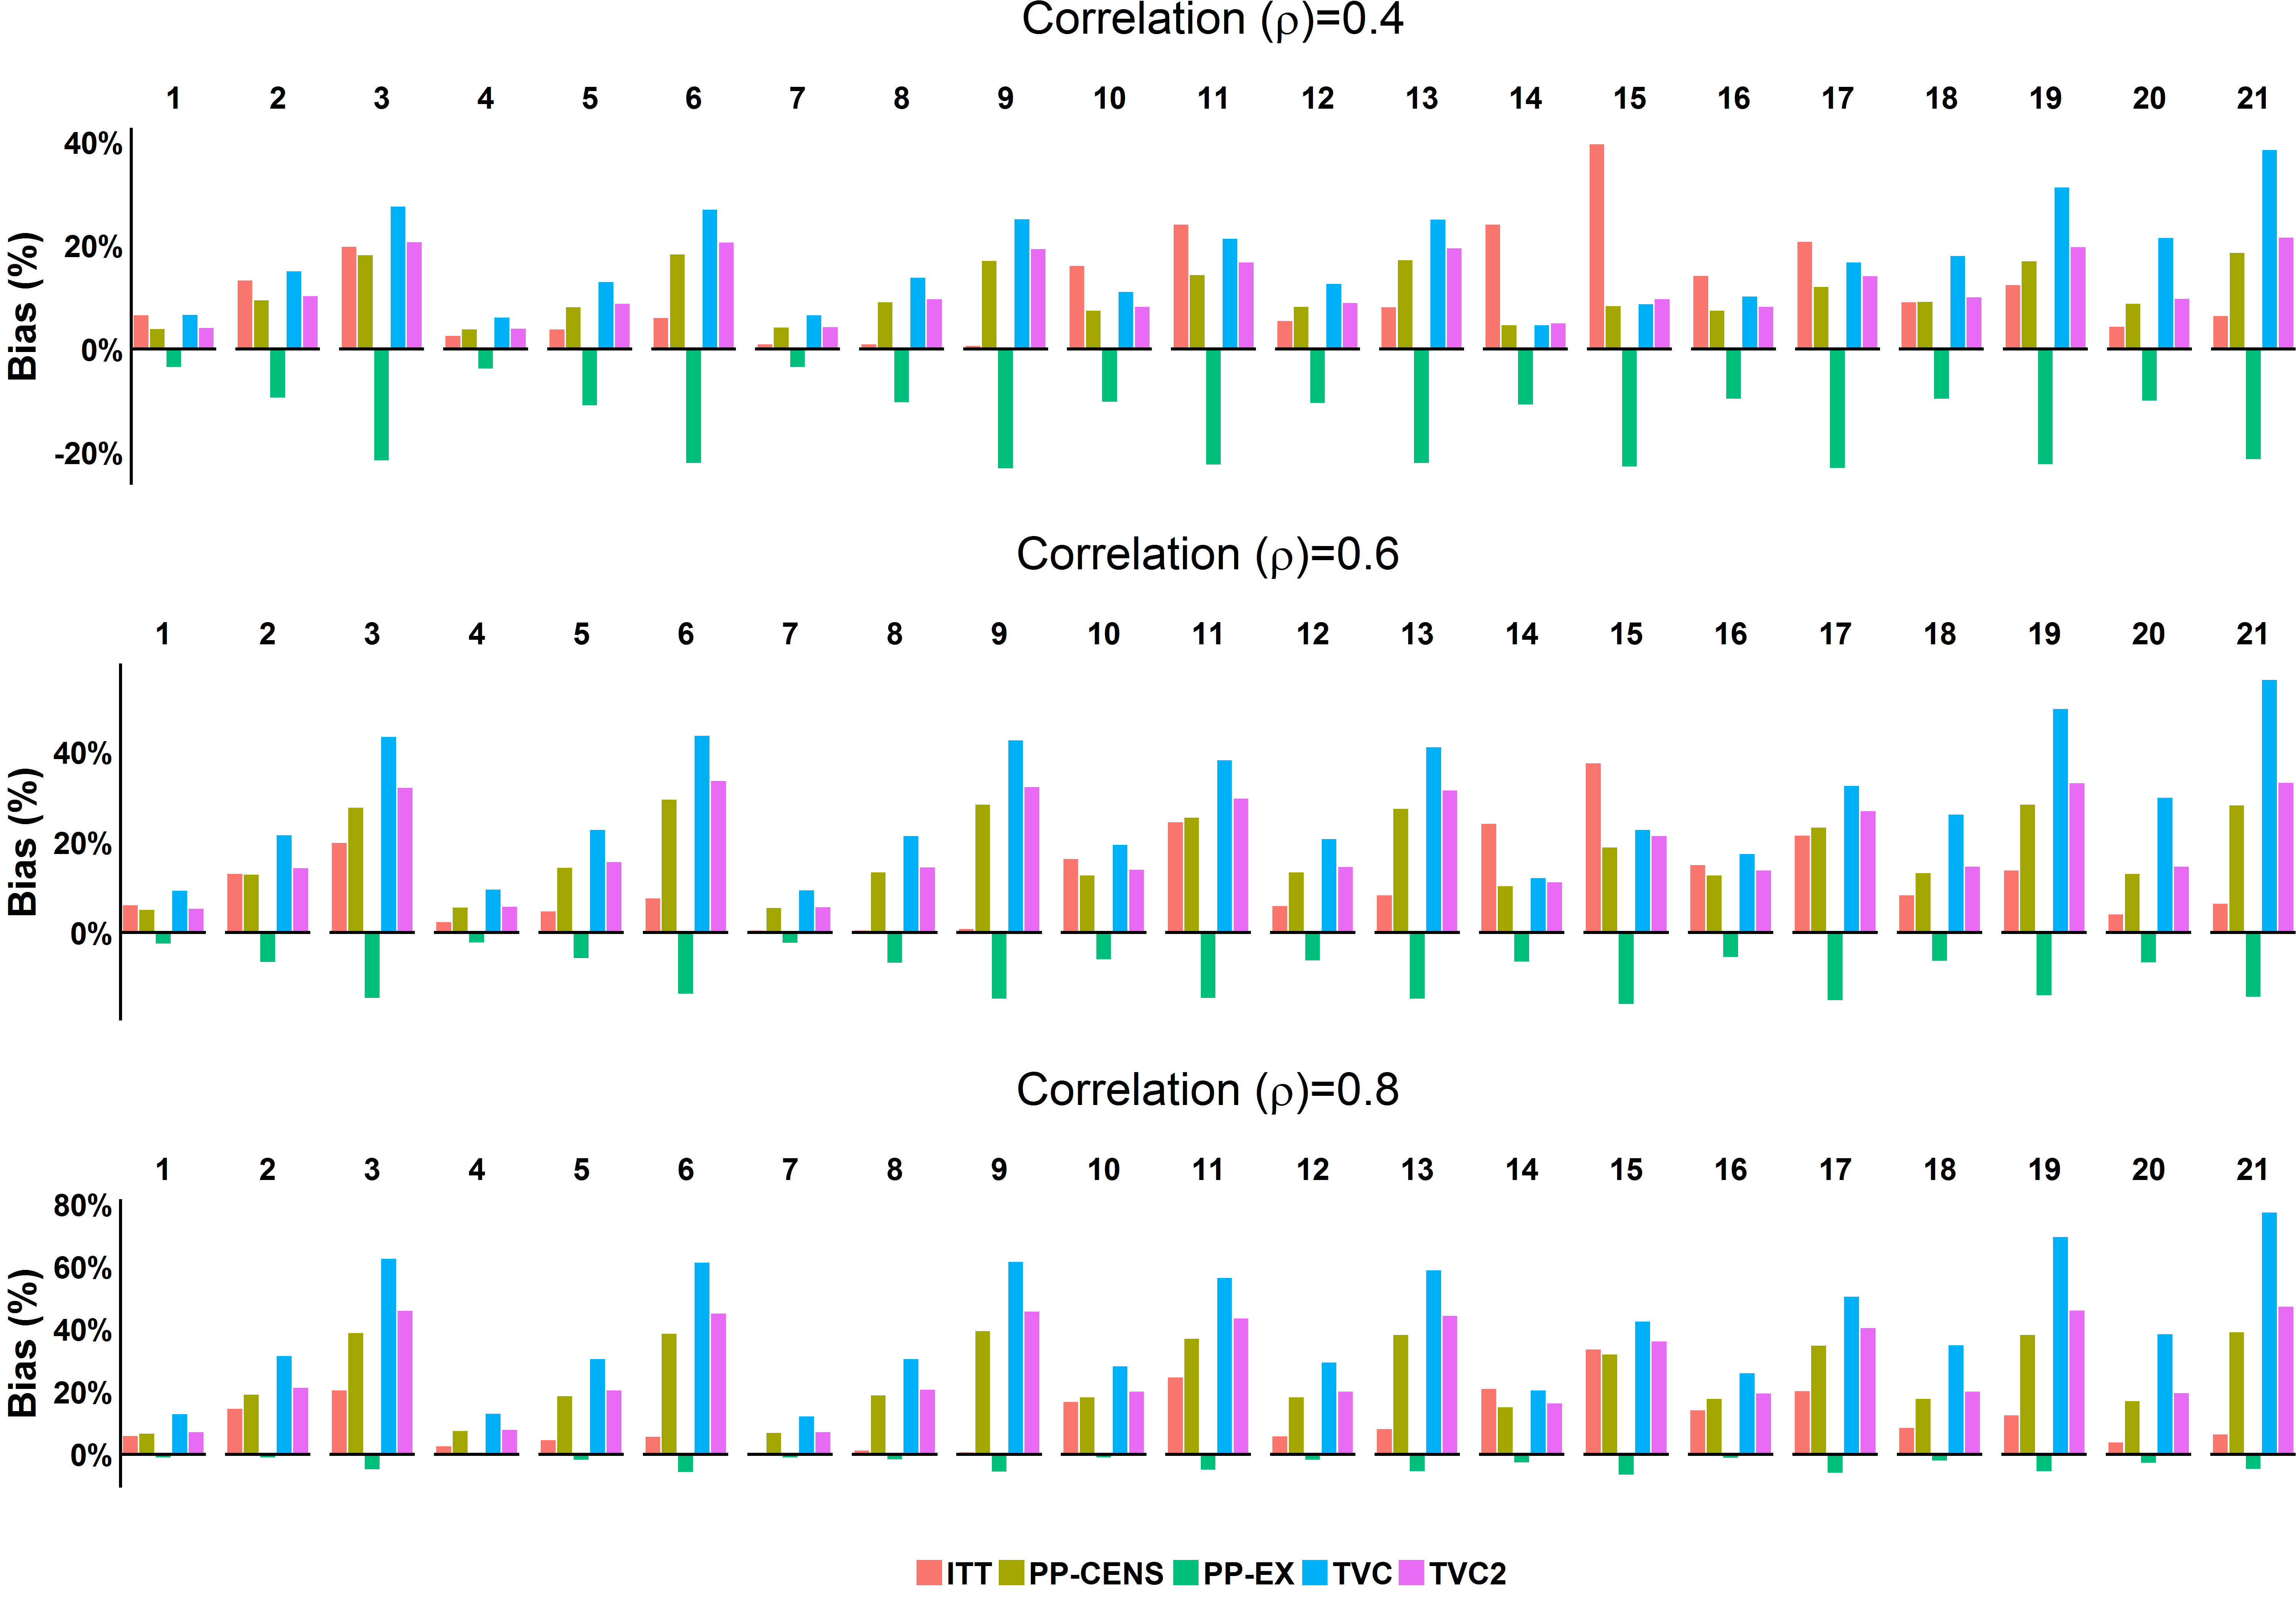
\includegraphics[width=20cm]{images/app_allres/simp_bias4.png}
    \caption{The percentage bias across all simulations for the simple methods. \\ ITT = Intent to treat analysis; PP-CENS = Per-protocol censoring at switch; PP-EX = Per-protocol excluding switchers; TVC = Treatment as a time-varying covariate; TVC2 = Switch treatment as a time-varying covariate}
    \label{F:allp:simple}
\end{sidewaysfigure}

\begin{sidewaysfigure}
    \centering
    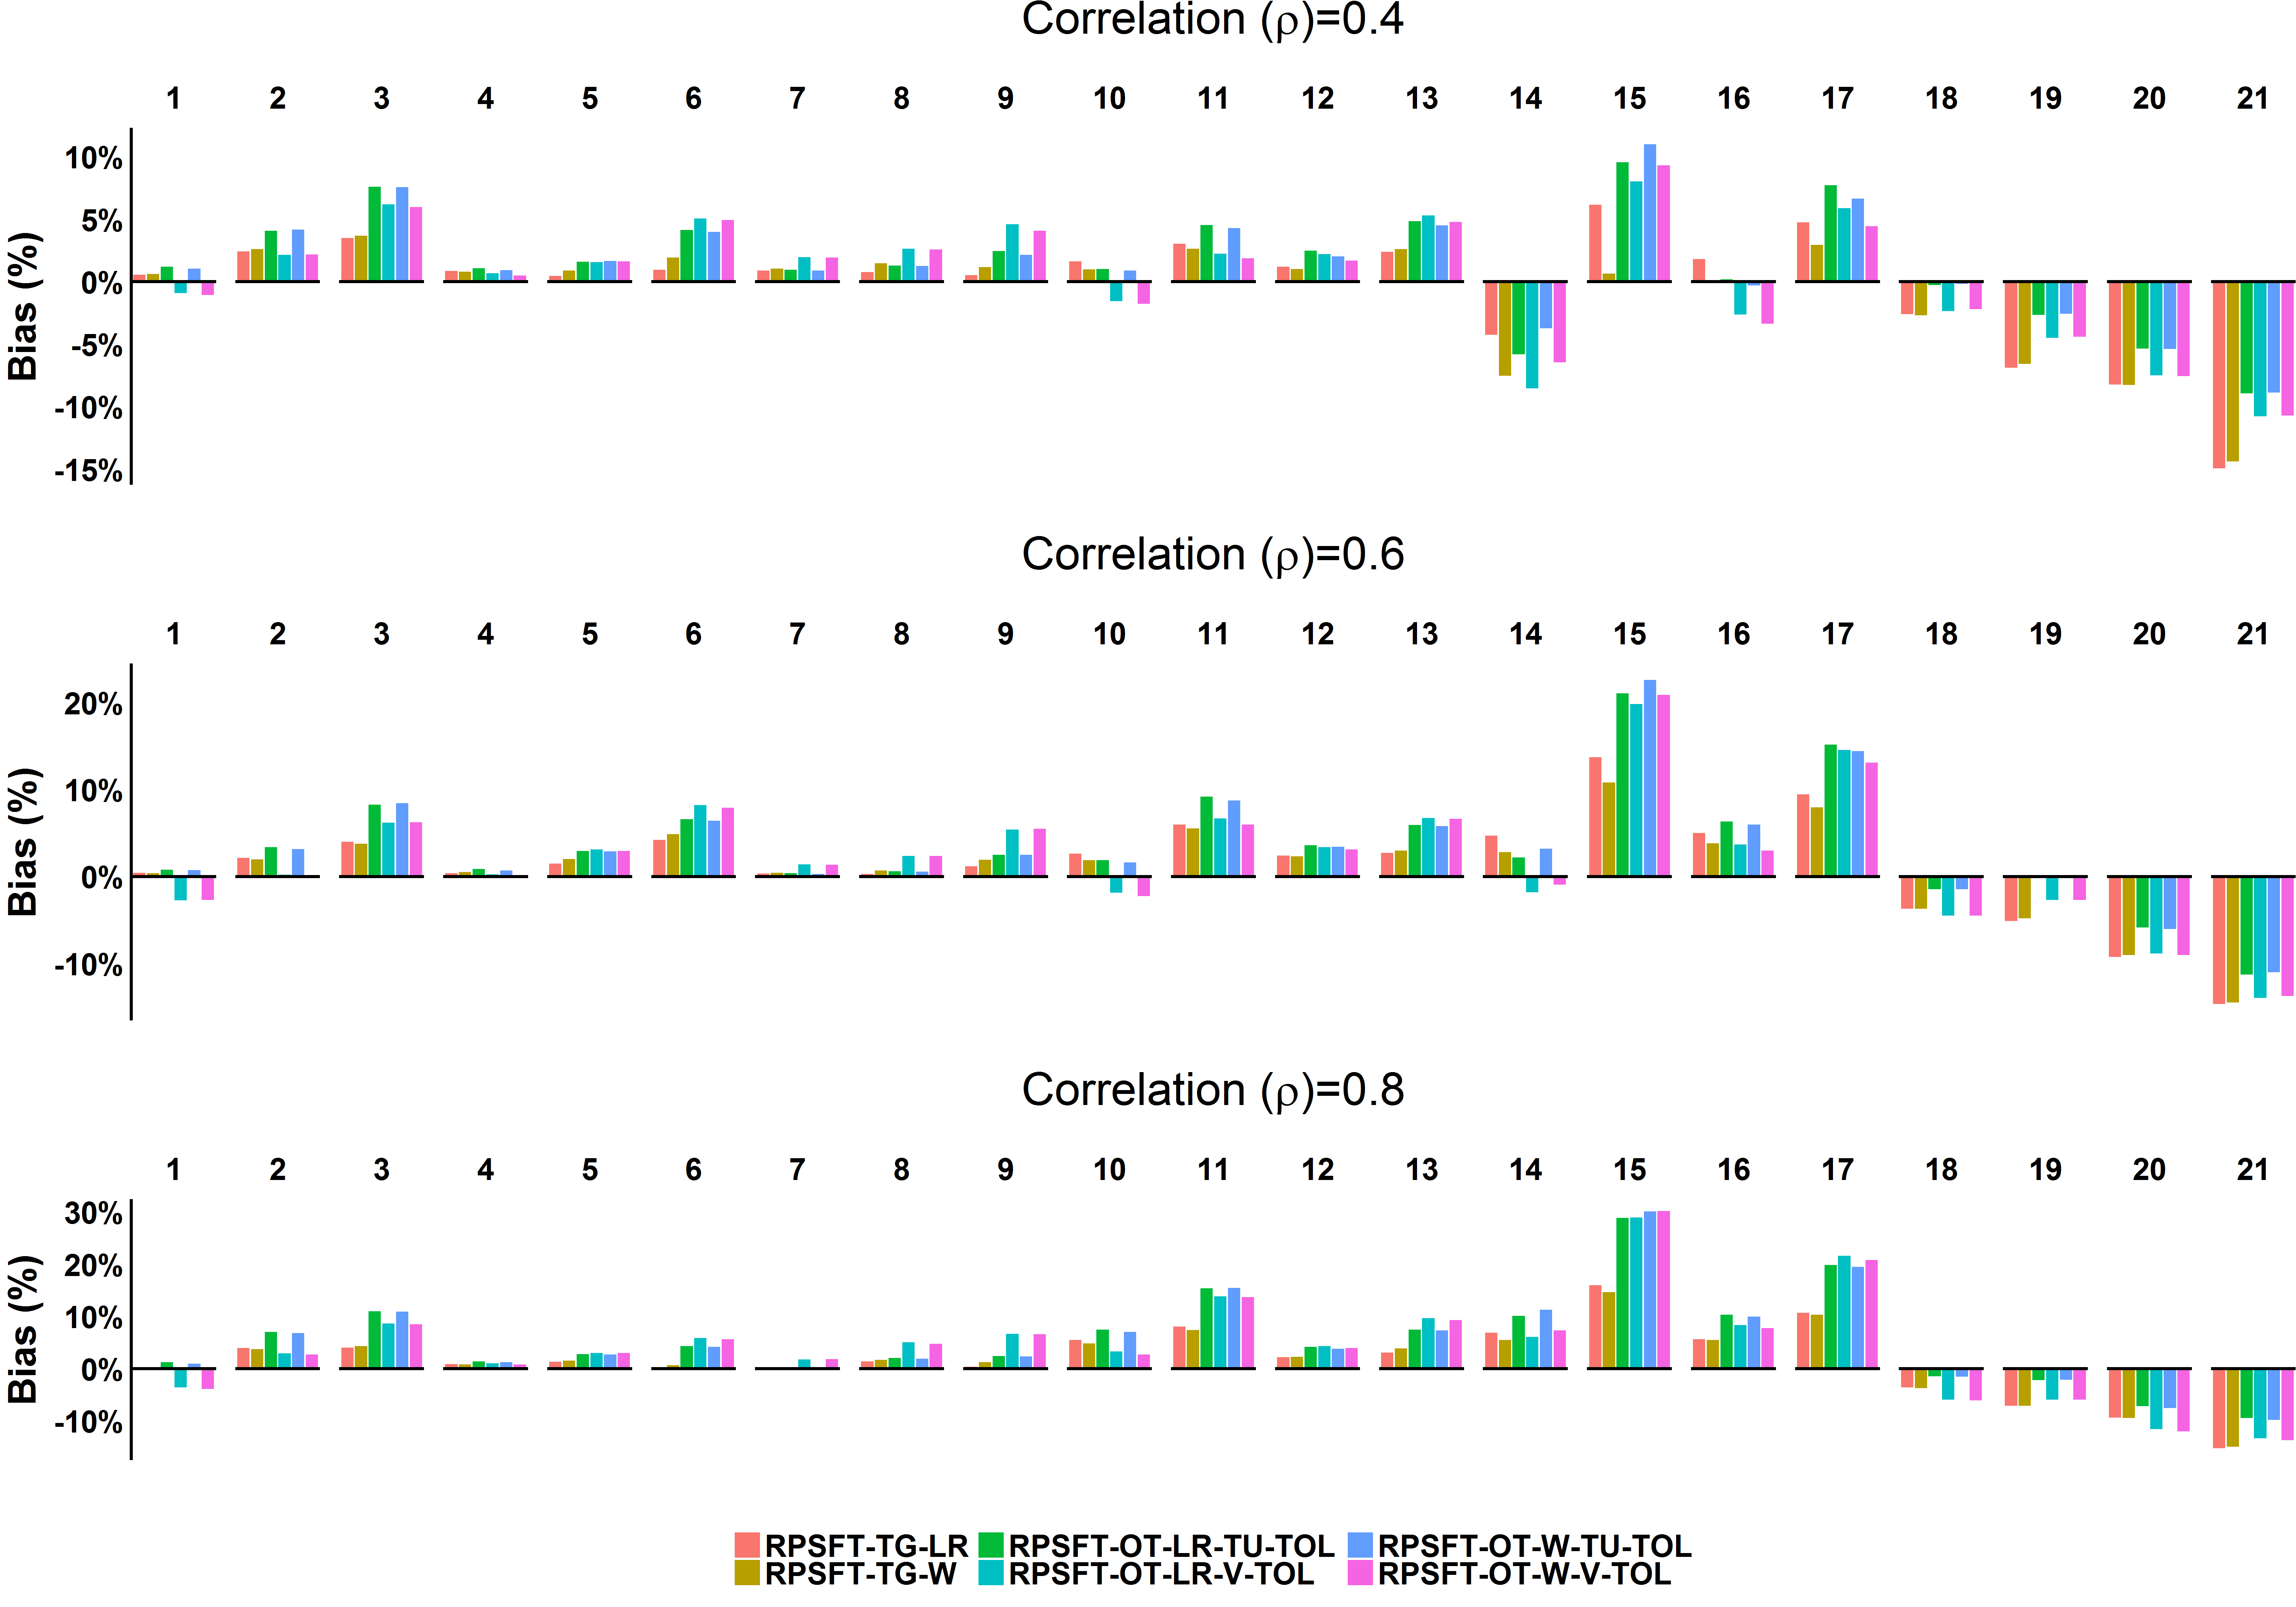
\includegraphics[width=20cm]{images/app_allres/rpsft_bias4.png}
    \caption{The percentage bias across all simulations for variations on the RPSFT method. \\ TG = ``treatment group''; OT = ``on treatment''; LR = log-rank test; W = wilcoxon test; TU = hazard ratio estimated as observed vs latent; V = hazard ratio estimated as counterfactual vs latent}
    \label{F:allp:rpsft}
\end{sidewaysfigure}

\begin{sidewaysfigure}
    \centering
    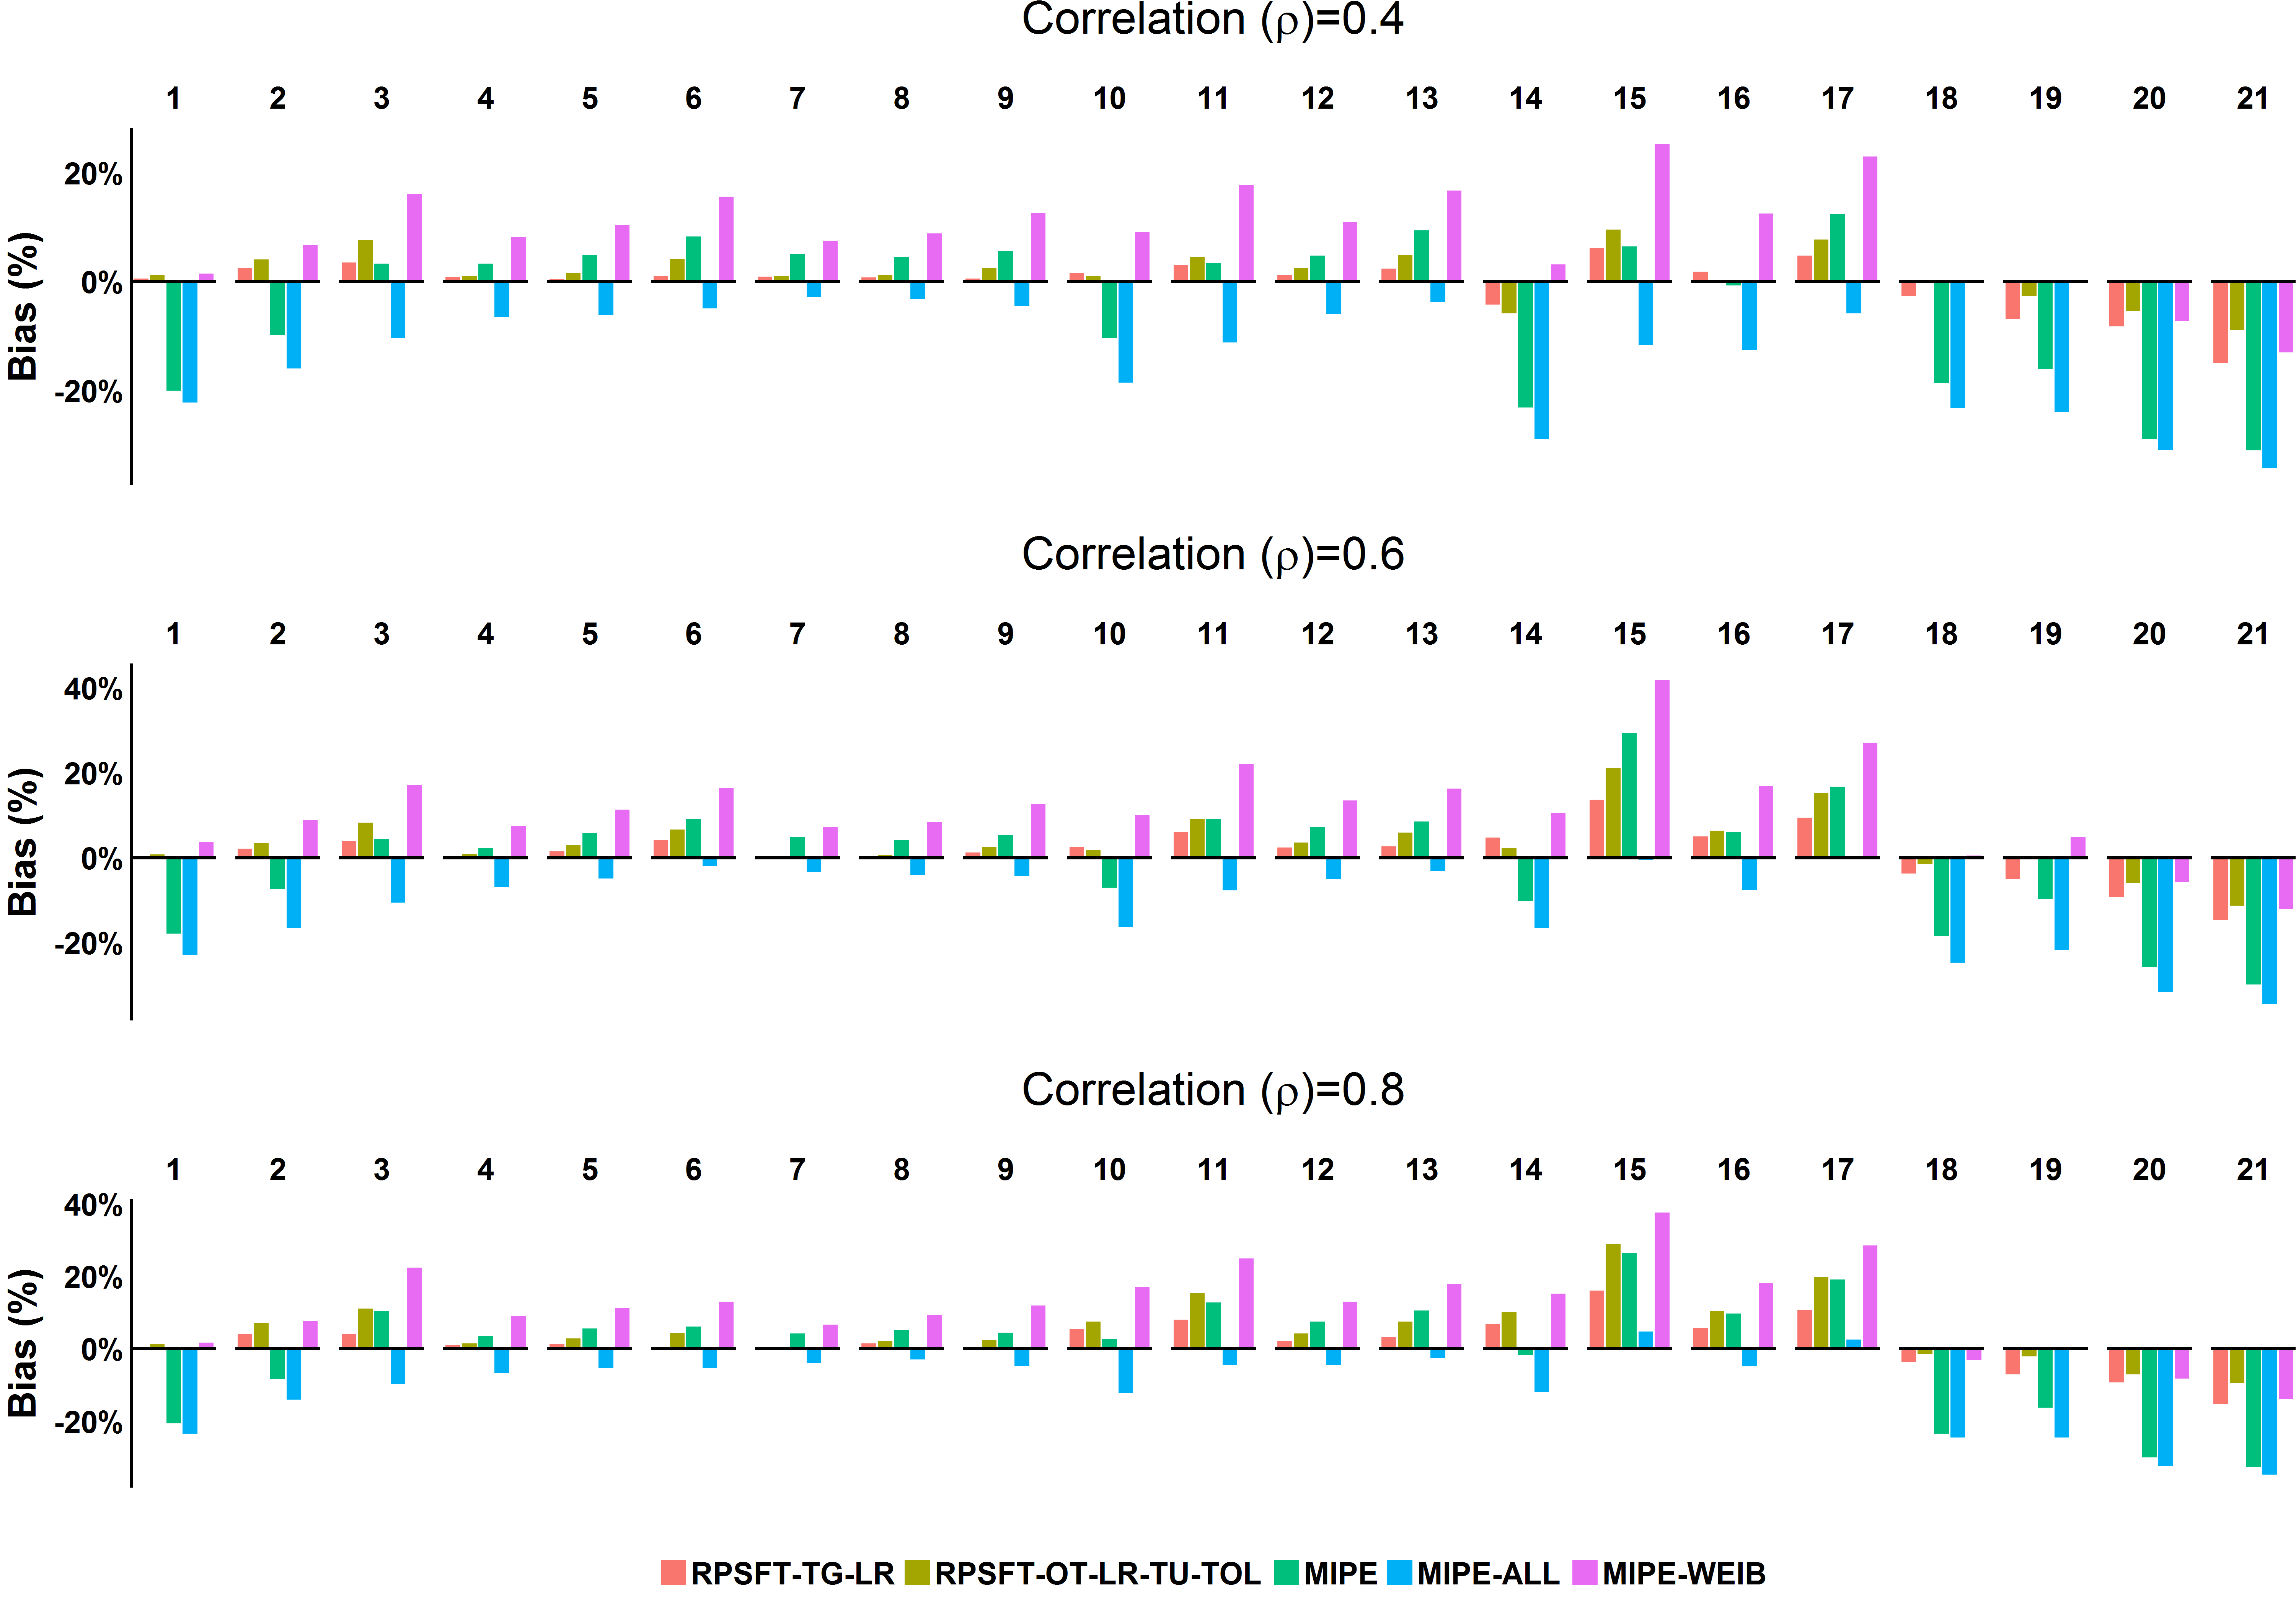
\includegraphics[width=20cm]{images/app_allres/mipe_bias4.png}
    \caption{The percentage bias across all simulations for the MIPE method compared to the RPSFT method. \\ MIPE = modified iterative parameter estimation; MIPE-ALL = imputations for non convergence; MIPE-WEIB = hazard ratio taken from weibull estimation;  TG = ``treatment group''; OT = ``on treatment''; LR = log-rank test}
    \label{F:allp:mipe}
\end{sidewaysfigure}

\begin{sidewaysfigure}
    \centering
    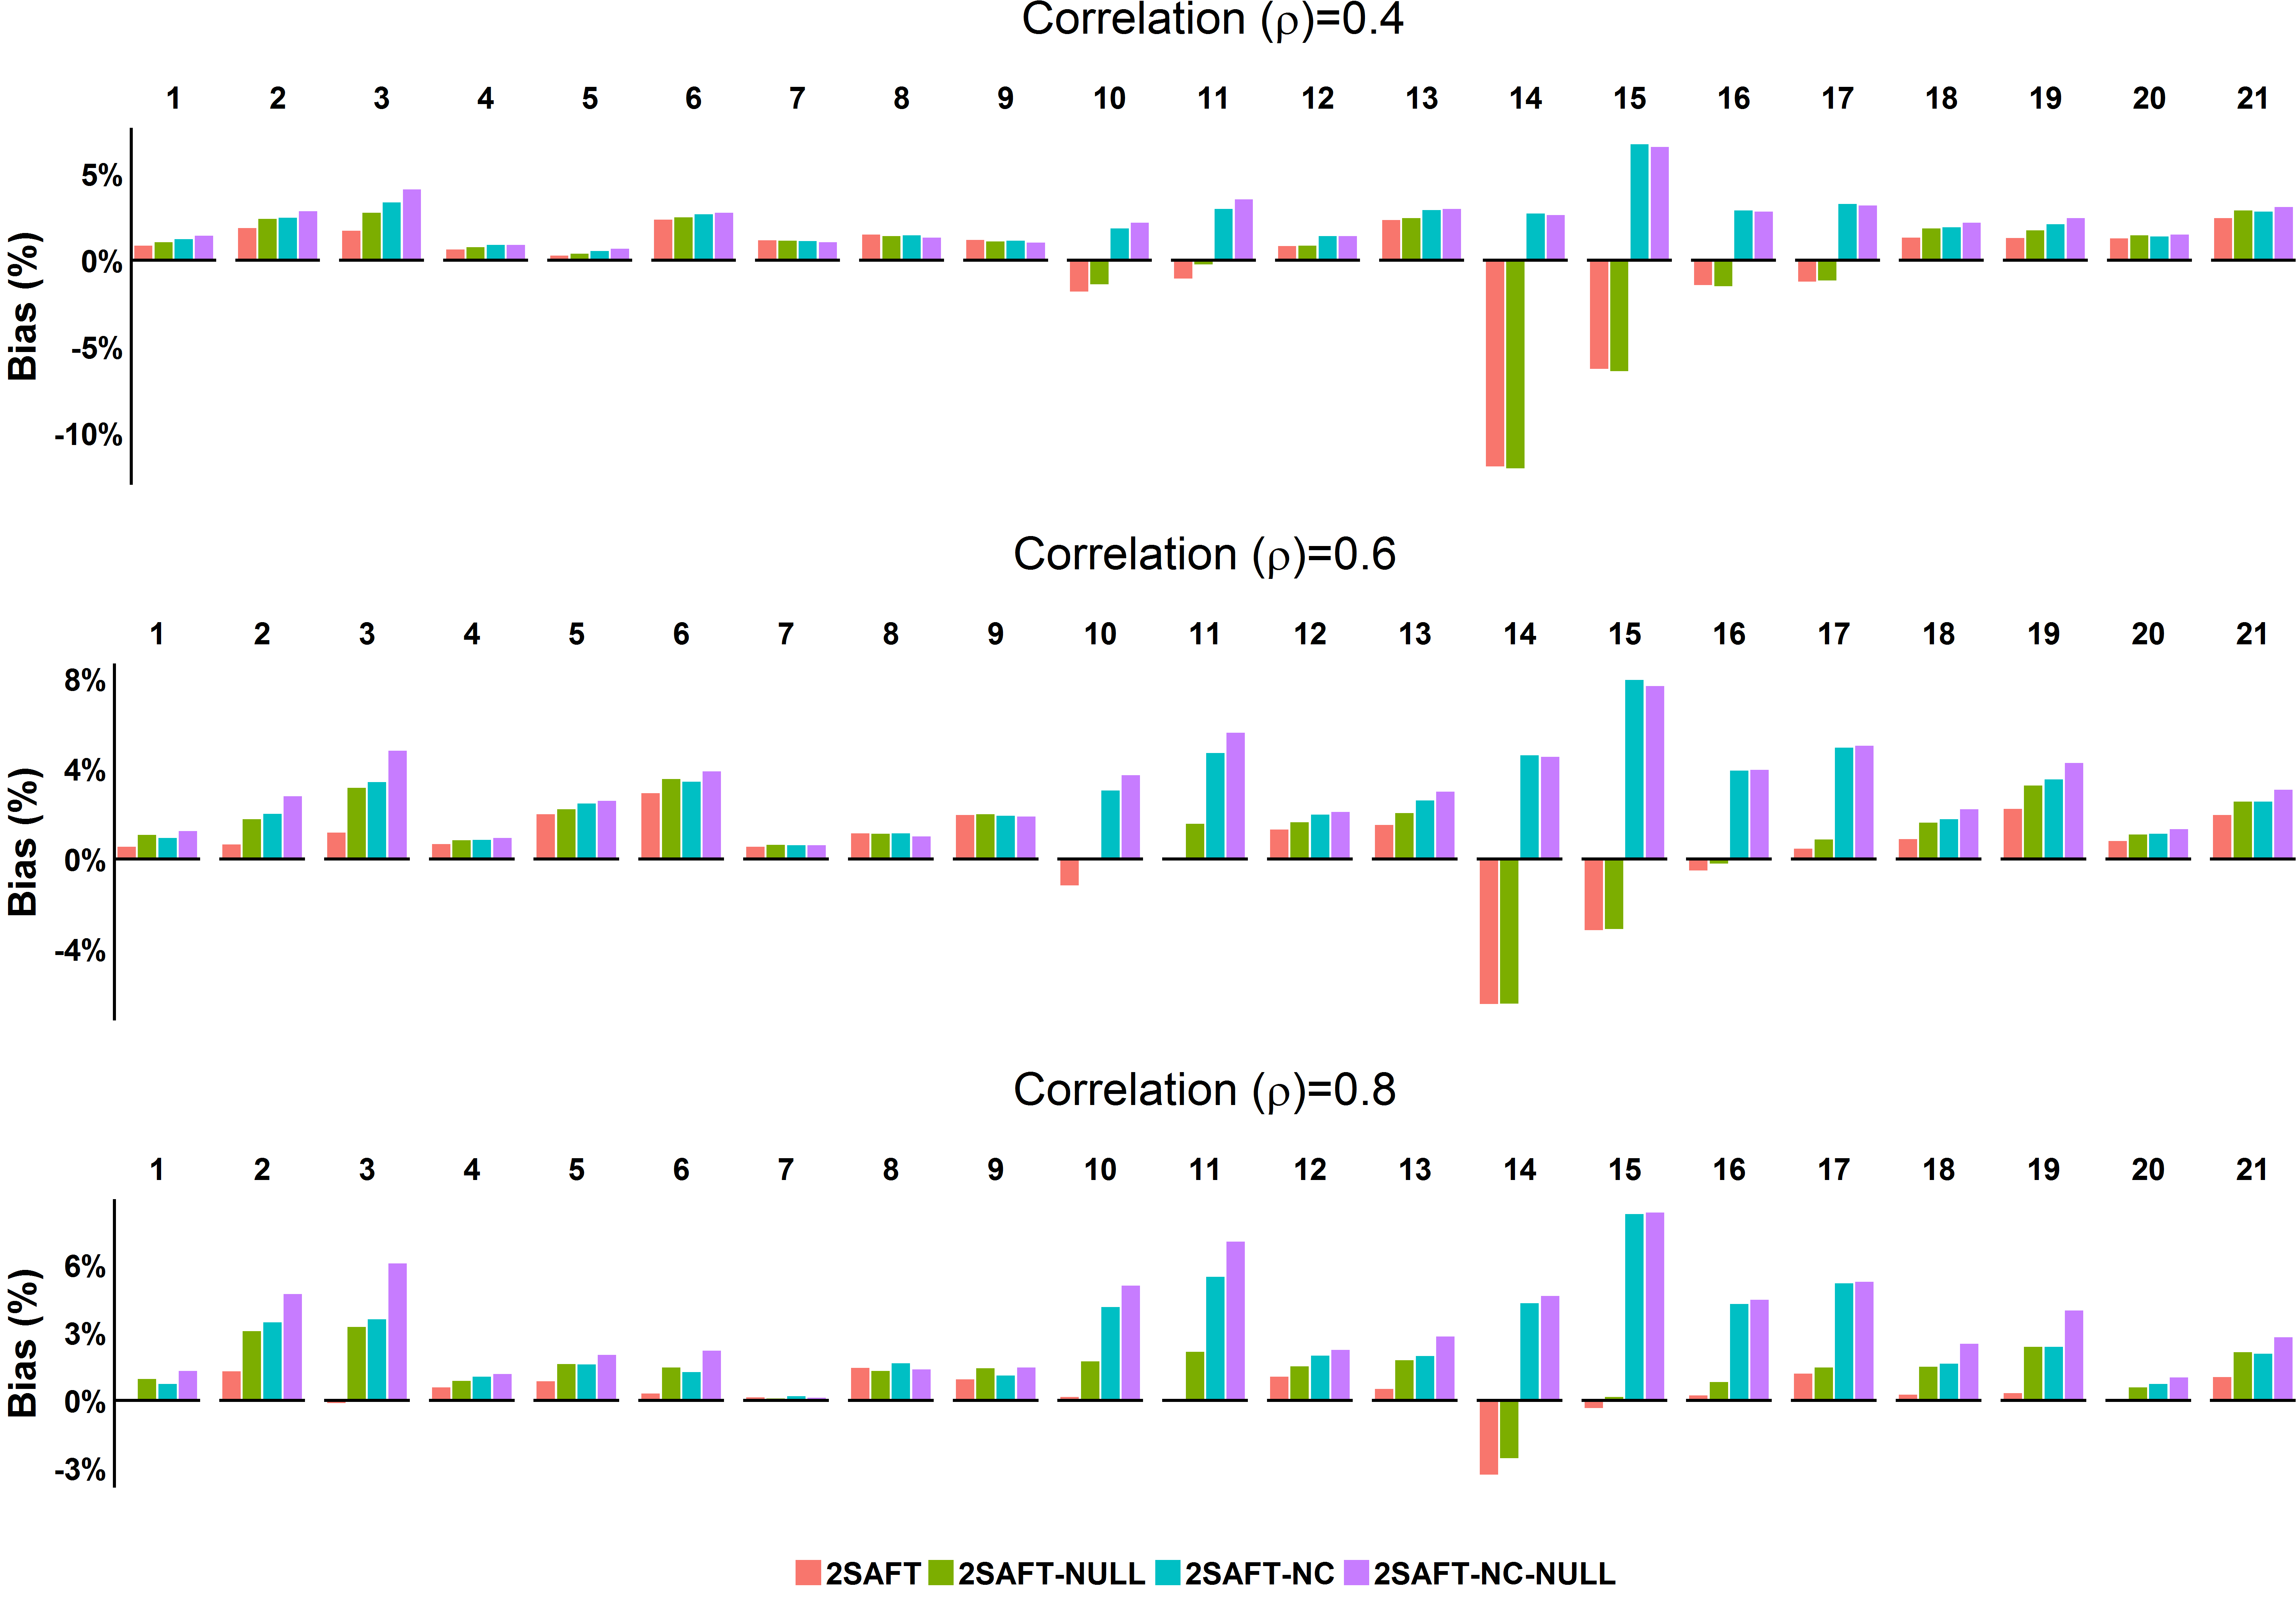
\includegraphics[width=20cm]{images/app_allres/saft_bias4.png}
    \caption{The percentage bias across all simulations for the Two Stage AFT method. \\ 2SAFT = including PFS as a covariate; 2SAFT-NULL = model with no covariates; NC = no recensoring}
    \label{F:allp:saft}
\end{sidewaysfigure}
